\section{Discrete Random Variables}
\begin{itemize}
  \item A \underline{discrete random variable} associates a real number
    with each outcome in $\Omega$, e.g., $X = i$ is a random variable
    if the throw of a die is $i$ for $i = 1,2,\ldots,6$.
  \item Note that $X^2$ is still a random variable and in general,
    a function of a random variable is also a random variable.
  \item \underline{Probability mass function} is the set
    $\{a, P_X(a)\}$ where $a \in \mathcal{A}$ and $\mathcal{A}$ is the
    set of all possible values taken by $X$.
\end{itemize}
\begin{example}
  Chess match between Alice and Bob. The first to win a game wins the
  match and conversely, the match is drawn if there are $10$ consecutive
  draws.
  \begin{equation*}
    P(\text{Alice wins a game}) = 0.3 \qquad
    P(\text{Bob wins a game}) = 0.4 \qquad
    P(\text{Draw}) = 0.3
  \end{equation*}
  \begin{enumerate}
    \item What is the PMF of the duration of a match?

      Let $L$ denote the duration of the match. Suppose $L=10$, then
      \begin{equation*}
        P_L(10) = (0.3)^9
        .
      \end{equation*}
      Otherwise, if $L = k < 10$,
      \begin{equation*}
        P_L(k) = (0.3)^{k-1} (0.7) \quad \text{for }\ k=1,2,\ldots,9
        .
      \end{equation*}
    \item Calculate $P(\text{Alice wins the match})$.
      \begin{align*}
        P(\text{Alice wins the match}) &= (0.3) + (0.3)(0.3) + \ldots
        + (0.3)^9(0.3) \\
        &= \sum_{k=0}^{9} (0.3)^k(0.3)
      \end{align*}
    \item Assuming no limit to the number of games played, find
      $P(\text{Alice wins the match})$ again.
      \begin{enumerate}
        \item $P(\text{Alice wins the match}) = \sum_{k=0}^{\infty} (0.3)^k(0.3) = (0.3) \sum_{k=0}^{\infty} (0.3)^k = \frac{0.3}{1-0.7} = \frac{3}{7}$
      \end{enumerate}
  \end{enumerate}
\end{example}
\begin{itemize}
  \item \underline{Functions of a RV:}

    Let $P_X(x) = 0.2 \quad x=-2,-1,0,1,2$.
    \begin{center}
      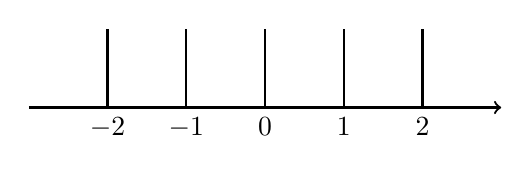
\begin{tikzpicture}
        \draw[thick,->] (0,0) -- (6,0);
        \draw[thick] (1,0) -- (1,1) node[below] at (1,0) {$-2$};
        \draw[thick] (2,0) -- (2,1) node[below] at (2,0) {$-1$};
        \draw[thick] (3,0) -- (3,1) node[below] at (3,0) {$0$};
        \draw[thick] (4,0) -- (4,1) node[below] at (4,0) {$1$};
        \draw[thick] (5,0) -- (5,1) node[below] at (5,0) {$2$};
      \end{tikzpicture}
    \end{center}
\end{itemize}
